% !TeX root = main.tex
% !TeX TXS-program:compile = txs:///pdflatex/[--shell-escape]

% Dokumenteneinstellungen
% !TeX root = ..\main.tex

% Papierformat
\documentclass[a4paper, 12pt]{report}

% Sprache
\usepackage[ngerman]{babel}
\usepackage{hyphenat}
% Bsp.: \hyphenation{Mathe-matik wieder-gewinnen}

% Seitenränder
\usepackage[a4paper,left=3cm,right=3cm,top=3cm,bottom=3cm]{geometry}

% Schriftpakete
\usepackage{tabularx}       % Dynamische Tabellen
\usepackage{multirow}       % Mehrere Zeilen untereinander zusammenfassen
\usepackage[utf8]{inputenc}	% Benutze UTF8 Zeichen
\usepackage[T1]{fontenc}	% Bessere Wort-Trennung
\usepackage[scaled]{helvet} % Skalierte Helvetica-Schriftart (serifenfrei)
\usepackage[gen]{eurosym}   % Eurosymbol '€'
% \usepackage{underscore}     % Unterstriche mit '_' anstatt '\_' schreiben
\usepackage{lmodern}        % Latin Modern -> schönere Schrift in PDF-Files
\usepackage{microtype}      % Mikrotypografische Einstellungen verbessern
% 	\usepackage{textcmds}       % Englische Anführungszeichen
\usepackage{seqsplit}

\setlength {\marginparwidth }{2cm} % Prevent Issues with todonotes
\usepackage[colorinlistoftodos,prependcaption,textsize=tiny]{todonotes}
\usepackage{colortbl}
\usepackage{xltabular}

% Eineinhalbfacher Zeilenabstand
\usepackage[onehalfspacing]{setspace}

\usepackage{tocloft}

% Literaturverzeichnis
\usepackage[sorting=none, backend=bibtex, style=numeric]{biblatex}
\usepackage{xurl}

% Quellcode einbinden
\usepackage{ifthen}	  % IF-THEN Befehle
\usepackage{listings} % Quellcode anzeigen
\usepackage{textcomp} % Straight Single quotes in listings

% Mathematik
\usepackage{amsmath}  % Mathematische Funktionen
\usepackage{amsfonts} % Mathematische Schrift
\usepackage{amssymb}  % Mathematische Symbole
\usepackage{tikz}	  % Grafische Zeichnungen mit Linien, Punkten, Kurven, Rechtecken, ...
\usepackage[outline]{contour} % Pfeile fett machen
% \usepackage{minted} pygmentize not working on Windows

% Abkürzungsverzeichnis
\usepackage{acronym}
\usepackage{titlesec}

% Weitere Pakete
\usepackage{float}        % Floating objects wie figures oder tables
\usepackage{graphicx}     % Bilder/Grafiken
\usepackage{svg}		  % SVG (Skalierbare Vektorgrafiken) als Bildformat
\usepackage{pdfpages}     % PDF-Seiten/PDF-Dokumente einbinden
%\usepackage{filecontents} % Externe Files generieren
\usepackage{url}	  	  % Anzeige von URLs
\usepackage{fancyhdr} 	  % Kopf- und Fußzeile manipulieren
\usepackage{caption}      % Bildunterschrift
\usepackage{csquotes}     % Quotes
\usepackage{xpatch}
\usepackage{xcolor}
\usepackage{realboxes}

% Verweis-Einstellungen
\usepackage[colorlinks=true, % Blöcke ausblenden, Verweise farbig markieren
linkcolor=black, % Abkürzungs-Links in schwarz
citecolor=black, % Zitat-Links      in schwarz
urlcolor=blue]   % URL-Links        in blau
{hyperref}	     % Einbinden von URL

%Dokumenteneinstellung
% Kopf- und Fußzeile
\fancypagestyle{fancy-style}{% Own style
	\fancyhf{}% Clear header and footer
	\fancyhead[C]{\slshape\nouppercase{\rightmark}}
%		\fancyhead[LE,RO]{\slshape\nouppercase{\rightmark}}
%		\fancyhead[LO,RE]{\slshape\nouppercase{\leftmark}}
	\fancyfoot[C]{\sffamily\thepage}% Custom footer
	\renewcommand{\headrulewidth}{0.4pt}% Line at the header visible
%	   \renewcommand{\footrulewidth}{0.4pt}% Line at the footer visible
}

% Redefine the plain page style
\fancypagestyle{plain}{%
	\fancyhf{}%
	\fancyfoot[C]{\sffamily\thepage}%
	\renewcommand{\headrulewidth}{0pt}% Line at the header invisible
	\renewcommand{\footrulewidth}{0pt}% Line at the footer invisible
}

\pagestyle{fancy-style}

\titleformat{\chapter}[display]{\normalfont\sffamily\huge\bfseries}{\chaptertitlename\ \thechapter}{20pt}{\Huge}
\titleformat{\section}{\normalfont\sffamily\Large\bfseries}{\thesection}{1em}{}
\titleformat{\subsection}{\normalfont\sffamily\large\bfseries}{\thesubsection}{1em}{}
\titleformat{\subsubsection}{\normalfont\sffamily\normalsize\bfseries}{\thesubsection}{1em}{}

% Redefine content fonts in chapter, section, figure, table
\renewcommand{\cftchapfont}{\sffamily\bfseries}
\renewcommand{\cftsecfont}{}
\renewcommand{\cftfigfont}{Figure }
\renewcommand{\cfttabfont}{Table }

% Obere Trennlinie
\renewcommand{\headrulewidth}{0.4pt}   % obere Trennlinie
\setlength{\headheight}{14.5pt}        % Höhe der Kopfzeile

% Untere Trennlinie
%\renewcommand{\footrulewidth}{0.4pt}  % untere Trennlinie

% Einrücktiefe für Absätze
\setlength\parindent{24pt}			   % Einrück-Tiefe der ersten Zeile für alle folgenden Absätze

% Quellenverzeichnis
\addbibresource{chapters/literature.bib}
\renewcommand{\mkbibnamelast}[1]{\sffamily\MakeUppercase{#1}}
\renewcommand{\mkbibnamefirst}[1]{\sffamily\MakeUppercase{#1}}
\xpatchbibdriver{misc} % Komma statt Punkt nach Titel
{\usebibmacro{title}\newunit}
{\usebibmacro{title}\printunit{\addcomma\space}}{}{}

% Starte neue Seite für jede neue Chapter
\let\stdchapter\chapter
\newcommand{\npchapter}{\newpage\stdchapter}

% Starte neue Seite für jede neue Section
\let\stdsection\section
\newcommand{\npsection}{\newpage\stdsection}

% Zeilenumbruch bei URLs korrekt gestalten
%\makeatletter 
%\g@addto@macro\UrlBreaks{ 
	%	\do\a\do\b\do\c\do\d\do\e\do\f\do\g\do\h\do\i\do\j 
	%	\do\k\do\l\do\m\do\n\do\o\do\p\do\q\do\r\do\s\do\t 
	%	\do\u\do\v\do\w\do\x\do\y\do\z\do\&\do\1\do\2\do\3 
	%	\do\4\do\5\do\6\do\7\do\8\do\9\do\0\do\-\do\/\do\_\do\.} 
\expandafter\def\expandafter\UrlBreaks\expandafter{\UrlBreaks\do\a%
	\do\b\do\c\do\d\do\e\do\f\do\g\do\h\do\i\do\j\do\k\do\l\do\m\do\n%
	\do\o\do\p\do\q\do\r\do\s\do\t\do\u\do\v\do\w\do\x\do\y\do\z\do\&}

% Grafikpfad setzen
\graphicspath{{images/}}

% Sprache
\selectlanguage{english}

% Visio-Grafiken ohne Rand einbinden
\newcommand{\includevisio}[2][]{\includegraphics[clip, trim=0.7mm 0.7mm 0.7mm 0.7mm, #1]{#2}}

% Bildunterschriften - Quelle
\newcommand{\source}{\\ Source: }

\definecolor{codeGray}{rgb}{0.9,0.9,0.9}

% Setze als Programmiersprache HTML
\lstdefinestyle{myStyle}{
	breaklines=true,
	numbers=none, 
	escapeinside={\%*}{*)},
	basicstyle=\footnotesize\ttfamily,
	showstringspaces=false,
	keepspaces=true,
	identifierstyle=\color{black},
	backgroundcolor=\color{codeGray},
}
\lstset{style=myStyle, language = HTML}

\colorlet{punct}{red!60!black}
\definecolor{delim}{RGB}{20,105,176}
\colorlet{numb}{magenta!60!black}
\lstdefinelanguage{json}{
	upquote=true,
	literate=
	*{:}{{{\color{punct}{:}}}}{1}
	{,}{{{\color{punct}{,}}}}{1}
	{\{}{{{\color{delim}{\{}}}}{1}
	{\}}{{{\color{delim}{\}}}}}{1}
	{[}{{{\color{delim}{[}}}}{1}
	{]}{{{\color{delim}{]}}}}{1},
}
\lstdefinelanguage{java}{
	upquote=true,
	literate=
	*{;}{{{\color{DCLred}{;}}}}{1}
	{[}{{{\color{delim}{[}}}}{1}
	{]}{{{\color{delim}{]}}}}{1},
	morekeywords={encodedString},
	keywordstyle={\color{black}},
	morekeywords=[2]{String, byte, binary}, 
	keywordstyle=[2]{\color{delim}}
}

\colorlet{DCLmagenta}{punct}
\colorlet{DCLred}{red}
\colorlet{DCLblue}{blue}
\lstdefinelanguage{dcl}{
	upquote=true,
	literate =
	*{;}{{{\color{DCLred}{;}}}}{1}
	{0}{{{\color{DCLblue}{0}}}}{1}
	{1}{{{\color{DCLblue}{1}}}}{1}
	{2}{{{\color{DCLblue}{2}}}}{1}
	{3}{{{\color{DCLblue}{3}}}}{1}
	{4}{{{\color{DCLblue}{4}}}}{1}
	{5}{{{\color{DCLblue}{5}}}}{1}
	{6}{{{\color{DCLblue}{6}}}}{1}
	{7}{{{\color{DCLblue}{7}}}}{1}
	{8}{{{\color{DCLblue}{8}}}}{1}
	{9}{{{\color{DCLblue}{9}}}}{1}
	{[}{{{\color{DCLred}{[}}}}{1}
	{]}{{{\color{DCLred}{]}}}}{1},
	morekeywords={POLICY, DEFAULT, FUNCTION, TEST, SCHEMA},
	keywordstyle={\color{delim}},
	morekeywords=[2]{GRANT, IN, ON, WHERE, AND, OR, LIKE, BETWEEN, USE, IS, NOT, NULL, RETURN, DENY, INPUT, Number, String}, 
	keywordstyle=[2]{\color{DCLred}}
}


\makeatletter
\xpretocmd\lstinline{\Colorbox{codeGray}\bgroup\appto\lst@DeInit{\egroup}}{}{}
\makeatother

% Fortführende Absätze einrücken
\newcommand{\absatz}{\noindent\hspace*{12pt}}

\newcommand{\hash}[1]{\ttfamily\seqsplit{#1}}
\newcommand{\colorred}[1]{\textcolor{red}{#1}}
\newcommand{\colorblue}[1]{\textcolor{blue}{#1}}
\newcommand{\colorgreen}[1]{\textcolor{teal}{#1}}

\newcommand\tab[1][1cm]{\hspace*{#1}} % \tab-command

% Quellcode-Abbildungne
\usepackage{listings}
\usepackage{color}

\definecolor{lightgray}{rgb}{.9,.9,.9}
\definecolor{darkgray}{rgb}{.4,.4,.4}
\definecolor{purple}{rgb}{0.65, 0.12, 0.82}

\renewcommand{\lstlistingname}{Abbildung}
\lstdefinelanguage{JavaScript}{
	keywords={do, if, in, for, let, new, try, var, case, else, enum, eval, null, this, true, void, with, await, break, catch, class, const, false, super, throw, while, yield, delete, export, import, public, return, static, switch, typeof, default, extends, finally, package, private, continue, debugger, function, arguments, interface, protected, implements, instanceof},
	morecomment=[l]{//},
	morecomment=[s]{/*}{*/},
	morestring=[b]',
	morestring=[b]",
	ndkeywords={class, export, boolean, throw, implements, import, this},
	keywordstyle=\color{blue}\bfseries,
	ndkeywordstyle=\color{darkgray}\bfseries,
	identifierstyle=\color{black},
	commentstyle=\color{purple}\ttfamily,
	stringstyle=\color{red}\ttfamily,
	sensitive=true
}

\lstset{
	language=JavaScript,
	backgroundcolor=\color{lightgray},
	extendedchars=true,
	basicstyle=\footnotesize\ttfamily,
	showstringspaces=false,
	showspaces=false,
	numbers=left,
	numberstyle=\footnotesize,
	numbersep=9pt,
	tabsize=2,
	breaklines=true,
	showtabs=false,
	captionpos=b
}


% Alignment der Benchmark-Daten
\usepackage{siunitx} % Required for alignment
\sisetup{
	round-mode          = places, % Rounds numbers
	round-precision     = 4, % to 2 places
	locale              =DE,
	group-separator     = {.},
}

\begin{document}
	
% Titelseite
\begin{titlepage}
	\thispagestyle{empty}
	
	\begin{center}
		
\includegraphics[height=2.5cm]{logos/HKA_Logo.png}\\[16ex]
		\huge{\textbf{Evaluation von Bun 1.0: Eine Verbesserung der JavaScript-Laufzeitumgebung?}}\\[8ex]
		\large{Seminararbeit von}\\
		\large{Ansgar Lichter}\\[4ex]
		an der Fakult\"at f\"ur Informatik und Wirtschaftsinformatik\\[8ex]

		\begin{tabular}{lll}
			Universität:             & \quad Hochschule Karlsruhe     &       \\[2ex]
			Studiengang:             & \quad Informatik      &       \\[2ex]
			Professor:             & \quad Prof. Dr.-Ing. Vogelsang      &       \\[2ex]
			Bearbeitungszeitraum:      & \quad 01.10.2023 - 04.12.2023                                  &       \\[2ex]
		\end{tabular}
	\end{center}
\end{titlepage}

% Abstract
%% !TeX root = ..\main.tex
\titlespacing*{\chapter}{0pt}{0pt}{40pt}
\pagestyle{plain}
\chapter*{Abstract}
\addcontentsline{toc}{chapter}{Abstract}

\vfill
\titlespacing*{\chapter}{0pt}{50pt}{40pt}

% Inhaltsverzeichnis
\newpage
\pagenumbering{roman}
\setcounter{page}{2}
%\fancyhead[L]{\nouppercase{\leftmark}}
%\renewcommand{\contentsname}{Table of Contents}
\addcontentsline{toc}{chapter}{\contentsname}
\tableofcontents

% Abbildungsverzeichnis
\newpage
%\fancyhead[L]{\nouppercase{\leftmark}}
\addcontentsline{toc}{chapter}{\listfigurename}
\listoffigures

% Tabellenverzeichnis
\newpage
\phantomsection
\addcontentsline{toc}{chapter}{\listtablename}
\listoftables

% Abkuerzungsverzeichnis
\npchapter*{Abkürzungsverzeichnis}

\addcontentsline{toc}{chapter}{Abkürzungsverzeichnis}
\begin{filecontents}{miscellaneous/abbreviations.tex}

\end{filecontents}

\begin{acronym}
	\IfFileExists{miscellaneous/abbreviations-sorted}{\acro{api}[API]{Application Programming Interface}
\acro{crud}[CRUD]{Create, Read, Update, Delete}
\acro{jit-compiler}[JIT-Compiler]{Just-in-Time-Compiler}
\acro{lts}[LTS]{Long Term Support}
\acro{npm}[NPM]{Node Package Manager}
\acro{orm}[ORM]{Object-Relational Mapping}
\acrodef{jit-compiler-dativ-plural}[JIT-Compiler]{Just-in-Time-Compilern}
}{\acro{orm}[ORM]{Object-Relational Mapping}
\acro{api}[API]{Application Programming Interface}
\acro{jit-compiler}[JIT-Compiler]{Just-in-Time-Compiler}
\acrodef{jit-compiler-dativ-plural}[JIT-Compiler]{Just-in-Time-Compilern}
\acro{npm}[NPM]{Node Package Manager}
\acro{lts}[LTS]{Long Term Support}}
\end{acronym}

%cmd-Command zum Sortieren
%sort miscellaneous/abbreviations.tex /O miscellaneous/abbreviations-sorted.tex 

\pagestyle{fancy}
% Einleitung
% !TeX root = ..\main.tex
\pagestyle{fancy-style}
\npchapter{Einleitung}
\pagenumbering{arabic}

\section{Motivation}
JavaScript ist eine Programmiersprache, die vor allem im Kontext der Web-Entwicklung 
verwendet wird. Aktuell erfreut sich JavaScript großer Beliebtheit. 
In der Umfrage an Entwickler von Stack Overflow wurden mehr als 89.000 Entwickler 
befragt. JavaScript ist zum 11. Jahr in Folge die am häufigsten verwendete Programmiersprache. 
Mehr als 63\% der befragten Entwickler haben JavaScript als beliebteste Technologie 
gewählt. Bei den professionellen Entwicklern ist der Anteil mit mehr als 65\%
sogar noch höher. Außerdem ist TypeScript, eine stark typisierte Programmiersprache, die auf 
JavaScript aufbaut, unter den Teilnehmer auch beliebt. Ca. 39\% aller Entwickler und ca. 44\%
der professionellen Entwickler verwenden auch TypeScript. Damit ist TypeScript die 4. beliebteste 
Programmiersprache. Daraus folgt, dass das Ökosystem von JavaScript eine hohe Praxisrelevanz besitzt. \\

\noindent
JavaScript wird nicht nur für die Entwicklung im Frontend, sondern auch für die Entwicklung im Backend 
verwendet. Denn ungefähr 2\% der weltweit bekannten Server verwenden eine Laufzeitumgebung, die JavaScript 
ausführen kann. Die Laufzeitumgebung wird benötigt, um JavaScript außerhalb des Browsers ausführen zu können.
Hierbei ist Node.js die am weitesten verbreitete Laufzeitumgebung. In einer Umfrage zum Zustand der JavaScript
beantworteten ca. 71\% von 30.000 befragten Entwicklern, dass sie Node.js als Laufzeitumgebung regelmäßig verwenden.
Nur ca. 9\% der befragten Entwickler verwenden Deno und ca. 3\% Bun als eine Alternative zu Node.js. \\

\noindent
Node.js ist der Platzhirsch im Kontext von Laufzeitumgebungen von JavaScript. Dennoch besitzt Node.js Schwächen,
die die Alternativen versuchen zu lösen. Zu den Schwächen zählen eine schwächere Performance bei anspruchsvollen
Aufgaben, die Limitierung auf einen einzelnen Thread und häufige Änderungen an der API.


\section{Zielsetzung}
Zuvor wurde bereits Bun als Alternative zu Node.js genannt. Bun ist eine Laufzeitumgebung, die am 9. September 2023 in der Version 1.0 erschienen ist. Der Entwickler von Bun
haben das Ziel die Nachteile von Node.js zu lösen, damit das eigene Framework immer mehr verwendet wird.
Als Features werden eine hohe Verbesserung der Performance, elegante Schnittstellen und eine angenehme Erfahrung für Entwickler beworben.
Das Ziel dieser Arbeit ist es, Bun als eine Alternative zu Node.js zu evaluieren. Dazu werden die folgenden Leitfragen beantwortet: 
\begin{itemize}
    \item Welche Laufzeitumgebung besitzt die beste Performance?
    \item Ist Bun als Laufzeitumgebung kompatibel mit bestehenden Projekten auf der Basis von Node.js?
\end{itemize}
   
\section{Aufbau der Arbeit}
TODO




% Grundlagen
% !TeX root = ..\main.tex
\npchapter{Grundlagen} \label{ch:foundations}
Dieses Kapitel stellt die benötigten Grundlagen vor, die für das Verständnis der darauffolgenden Kapitel notwendig sind. Hierzu zählen die Vorstellung von Node.js und Bun sowie weitere Grundlagen zur Performance.

\section{Node.js} \label{sec:foundations-Node.js}
Node.js ist ein beliebtes Tool für eine Vielzahl an unterschiedlichen Projekten, darunter leichtgewichtige Webservices, dynamische Webanwendungen und Tools für die Kommandozeile. Es handelt sich um eine plattformunabhängige Open-Source-Laufzeitumgebung, die es ermöglicht, JavaScript außerhalb des Browsers auszuführen. Node.js verwendet die V8 JavaScript Engine von Google. Diese ist in C++ geschrieben und wird von Google Chrome verwendet. Durch den Einsatz dieser Komponenten erreicht Node.js eine hohe Performance, weshalb Unternehmen wie Netflix und Uber Node.js in ihren Softwareprojekten einsetzen.\cite{OpenJSFoundation.2022}\\

\begin{figure}[h]
	\centering
	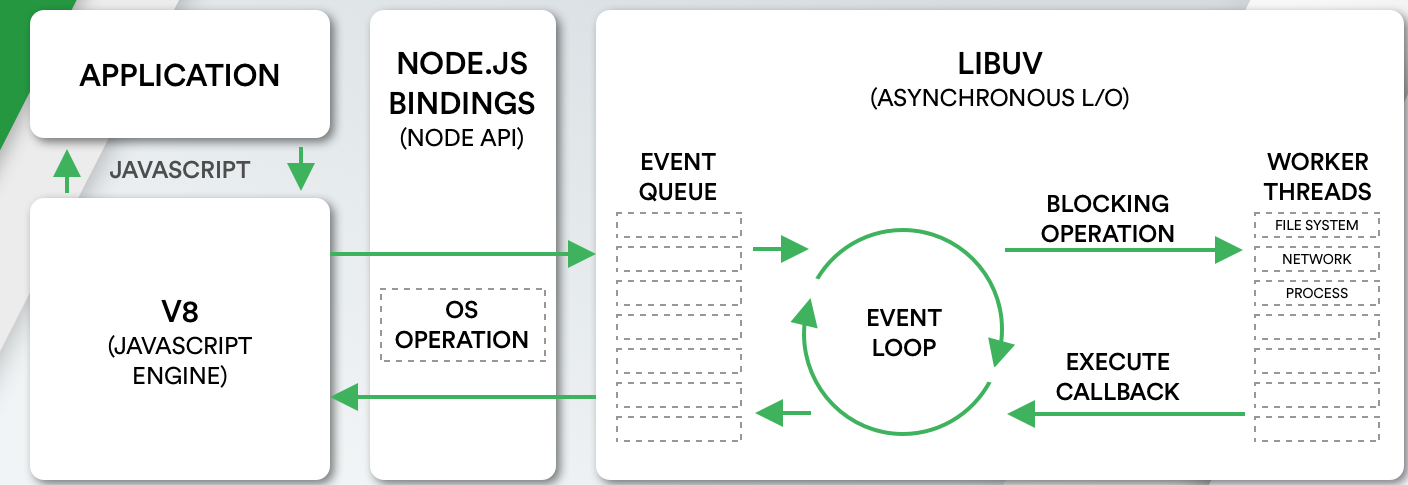
\includegraphics[width=\linewidth]{./images/NodeJsArchitecture}
	\caption{Node.js Architektur}
	\label{fig:nodejsArchitecture}
	\textit{Quelle: \cite{Kaneriya.2022}}
\end{figure}
 
\noindent
Wie in \autoref{fig:nodejsArchitecture} zu sehen, nutzt Node.js grundsätzlich nur einen Thread und erstellt nicht für jede neue Anfrage einen neuen Thread. Sobald eine Applikation gestartet wird, wird in dem erzeugten Thread der Node.js-Prozess gestartet. Die V8 Engine optimiert den Maschinencode an häufig benötigten Stellen, wobei dies nicht sofort geschieht, da die Übersetzung in Maschinencode aufgrund der Just-in-Time-Kompilierung eine zeitsensitive Aufgabe darstellt. Darüber hinaus ist in der Engine ein Garbage Collector integriert, der nicht mehr verwendete Objekte löscht.\cite{Springer.2022} \newline 
Für weitere Aufgaben setzt Node.js auf Bibliotheken, die fertige und etablierte Lösungsansätze für häufig benötigte Aufgaben zur Verfügung stellen. Nur für Aufgaben, für die keine etablierte Bibliothek existiert, werden eigene Implementierungen verwendet. Im Folgenden werden die wichtigsten Komponenten vorgestellt.\cite{Springer.2022}\\

\noindent
\textbf{Node.js Bindings} \newline
Node.js Bindings, auch bekannt als Node.js Add-ons, schaffen die Möglichkeit C- oder C++-Quellcode in Node.js zu integrieren. Entwickler können Erweiterungen in nativem Code erstellen und in ihren Anwendungen in JavaScript nutzen. Dies ermöglicht die Nutzung von Systemfunktionalitäten. Dies wird beispielsweise für den Zugriff auf das Dateisystem im Modul \glq fs\grq{} verwendet. Dieses ist in dem \ac{api} von Node.js enthalten. Darin bietet Node.js viele Lösungen für häufig benötigte Aufgaben, um die Entwicklung zu vereinfachen. Diese sind global im gesamten Anwendungscode verfügbar. Zu den globalen Objekten gehören beispielsweise \glq console\grq{} für die Ausgabe von Informationen in der Konsole und \glq Buffer\grq{} für den Umgang mit binären Daten. In der \ac{api} ist neben dem Modul \glq fs\grq{} beispielsweise das Modul \glq http\grq{} enthalten, um den Umgang mit dem HTTP-Protokoll zu vereinfachen. Die Module selbst sind in JavaScript geschrieben. Das heißt, der Kern von Node.js liegt in C (Libuv) und C++ (V8 Engine)  vor, die übrigen Komponenten sind in der Sprache der Plattform geschrieben. Allerdings ist in der Standard-API keine Unterstützung für TypeScript enthalten. Hierzu muss ein TypeScript-Compiler separat installiert werden.\cite{Springer.2022, OpenJSFoundation.2022b, OpenJSFoundation.o.J.b}\\

\noindent
\textbf{Event Loop} \newline
Node.js verwendet eine eventgesteuerte Architektur. Anstatt den Quellcode linear auszuführen, werden definierte Events ausgelöst, für die zuvor Callback-Funktionen registriert wurden. Dieses Konzept wird genutzt, um eine hohe Anzahl von asynchronen Aufgaben zu bewältigen. Lese- und Schreiboperationen werden an den Event Loop ausgelagert, um dabei den einzelnen Thread der Anwendung nicht zu blockieren. Wenn auf externe Ressourcen zugegriffen werden muss, leitet der Event Loop die Anfrage weiter und die registrierte Callback-Funktion gibt die Anfrage an das Betriebssystem weiter. In der Zwischenzeit kann Node.js andere Operationen ausführen. Das Ergebnis der externen Operation wird über den Event Loop zurückgeliefert.\cite{Springer.2022} \newline 
Während der Laufzeit werden viele Events erzeugt und in einer Message Queue, der Event Queue, nacheinander gespeichert. Node.js nutzt \glqq First In - First Out\grqq{} und beginnt demnach mit der Verarbeitung der ältesten Events und arbeitet sich durch die Queue, bis keine Events mehr vorhanden sind.\cite{OpenJSFoundation.o.J.c}\\

\noindent
\textbf{\glq Libuv\grq{}} \newline
Der Event Loop von Node.js basiert ursprünglich auf der Bibliothek \glq libev\grq{}. Diese ist in C geschrieben und für ihre hohe Leistung und umfangreichen Features bekannt. Allerdings stützt sich \glq libev\grq{} auf native UNIX-Funktionen. Diese sind auf Windows über eine andere Schnittstelle nutzbar. Daher dient \glq libuv\grq{} als Abstraktionsebene zwischen Node.js, libev und der Windows-Schnittstelle. Dadurch sind der Event Loop und die Laufzeitumgebung auf allen Plattformen lauffähig. \glq Libuv\grq{} verwaltet alle asynchronen I/O-Operationen, einschließlich Dateisystemzugriffe und asynchrone TCP- und UDP-Verbindungen.\cite{Springer.2022} \\

\noindent
\textbf{\ac{npm}} \newline
Der \ac{npm} ist entscheidend für den Erfolg von Node.js. Er wurde entwickelt, um die Abhängigkeiten in Projekten zu verwalten. Mittlerweile gibt es Pakete für eine Vielzahl an Anwendungsfällen. Denn im September 2021 existieren mehr als 2,1 Millionen Pakete. Der \ac{npm} ist nicht Teil des Executables von Node.js und wird deshalb bei der Installation häufig mitgeliefert. \cite{Springer.2022, OpenJSFoundation.2022b}\\

\noindent
Zusammenfassend zeichnet sich Node.js durch eine eventgesteuerte Architektur und durch ein nicht blockierendes Modell für Ein- und Ausgabeoperationen aus. Dadurch wird es leichtgewichtig und effizient. Dies hat verschiedene Vor- und Nachteile.\newline
Zu den Vorteilen gehören eine hohe Performance durch die Nutzung der V8 JavaScript Engine. Weitere Stärken sind die große und aktive Community an Entwicklern und die Plattformunabhängigkeit. Node.js ermöglicht die Verwendung der JavaScript-Sprache sowohl auf der Server- als auch auf der Clientseite. Dies vereinfacht die Entwicklung von Full-Stack-Anwendungen.\cite{Brown.November2019, OpenJSFoundation.2022b}\

\noindent
Allerdings existieren auch Nachteile bei der Verwendung von Node.js. Das Single-Thread-Modell kann bei rechenintensiven oder CPU-lastigen Aufgaben zu Engpässen führen, da es nur einen Hauptthread für die Ausführung der Anwendung gibt  \cite{Chhetri.2016}. Ein weiterer Nachteil ist, dass Node.js über eine begrenzte Standardbibliothek verfügt, sodass Entwickler häufig auf externe Module und Pakete zurückgreifen müssen, beispielsweise auf einen Transpiler für TypeScript \cite{OpenJSFoundation.2022b}.

\section{Bun} \label{sec:foundations-Bun}
Bun ist ein Open-Source-Toolkit für JavaScript. Dieses kombiniert verschiedene serverseitige Komponenten, um ein leistungsstarkes Paket zur Verfügung zu stellen. Bun ist auf MacOS und Linux für die produktive Nutzung freigegeben. Die Version von Windows besitzt aktuell einen experimentellen Status und ist noch nicht hinsichtlich der Performance optimiert. Alternativ kann auf Windows die veröffentlichte Linux-Version über das Windows Subsystem für Linux installiert werden. Ursprünglich ist Bun als ein persönliches Freizeitprojekt von Jared Sumner gestartet. Mittlerweile hat es sich zu einer wettbewerbsfähige Alternative zu bewährten Technologien in der Webentwicklung etabliert.\cite{Sumner.2023c, Tyson.2023}\\

\begin{figure}[!htb]
	\centering
	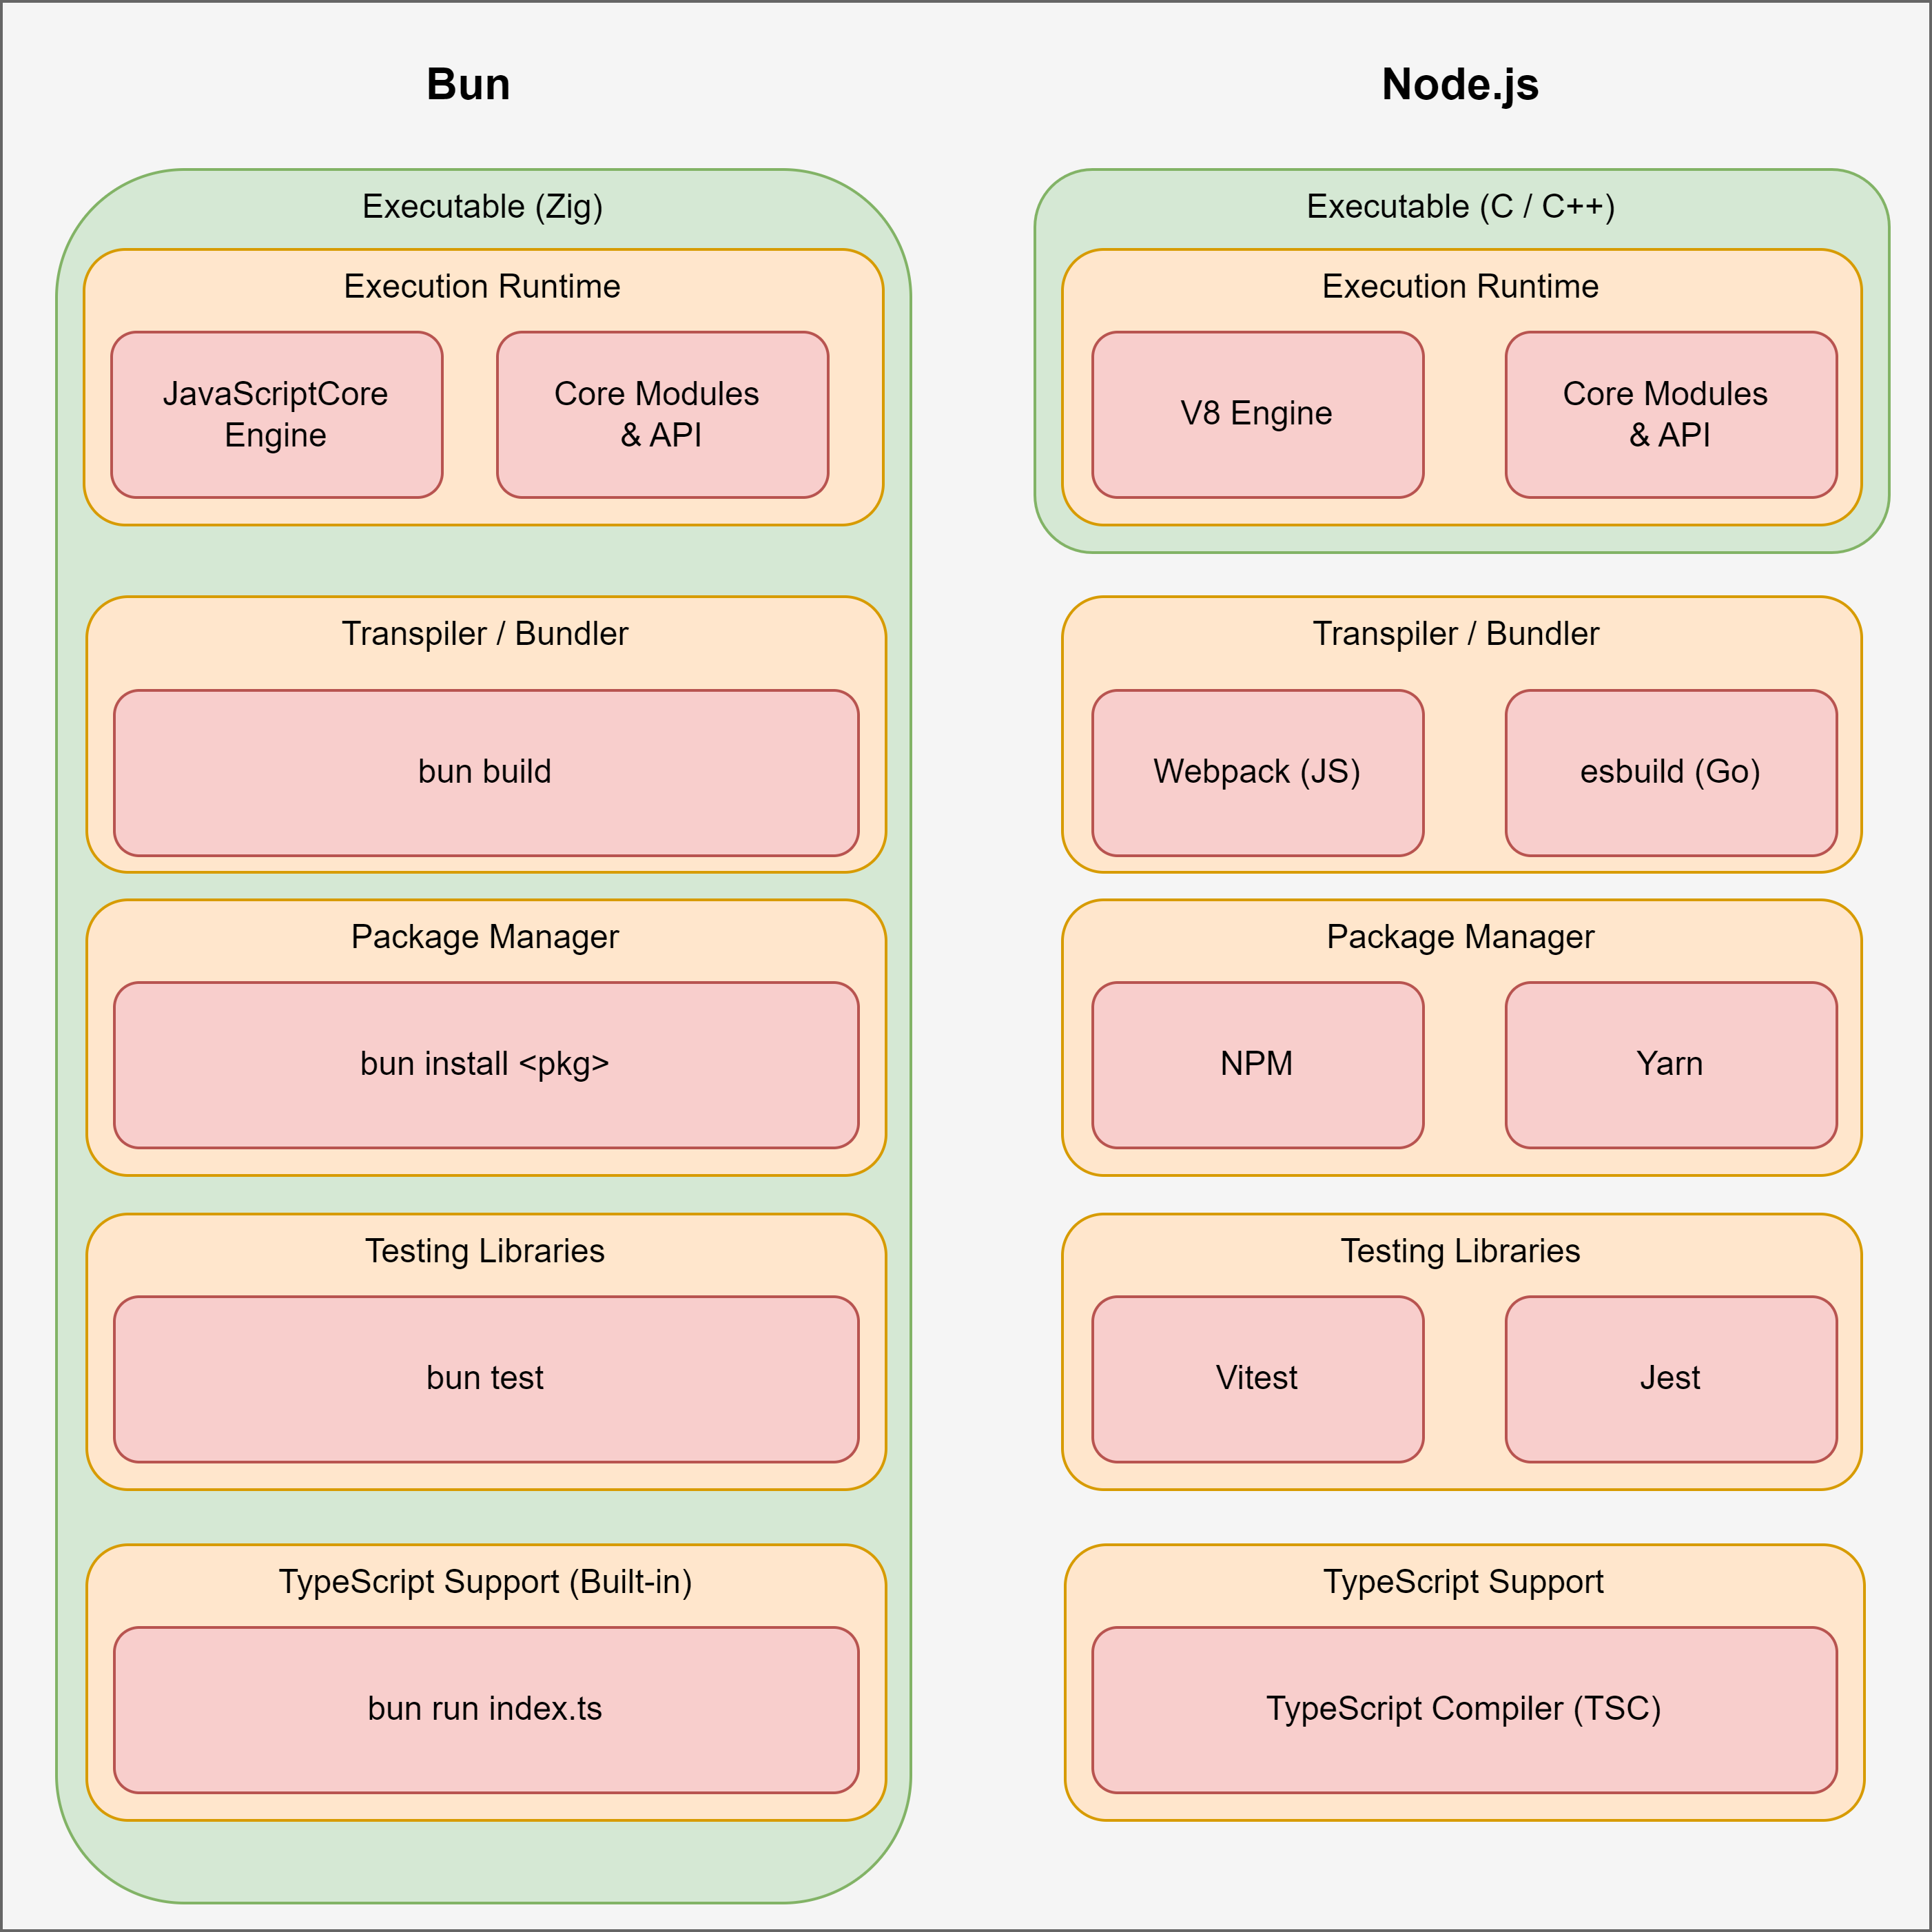
\includegraphics[width=\linewidth]{./images/EcosystemBunvsNode.png}
	\caption{Vergleich der Ökosysteme von Bun und Node.js}
	\label{fig:ecosystemComparison}
	\textit{Quelle: in Anlehnung an \cite{Springer.2022, OvenSh.2023c}}
\end{figure}

\noindent
\autoref{fig:ecosystemComparison} zeigt das Ökosystem von Bun im Vergleich zu Node.js. Im Toolkit von Bun sind folgende Komponenten enthalten:
\begin{itemize}
	\item eine Laufzeitumgebung für JavaScript,
	\item ein Paketmanager wie \ac{npm} (siehe \autoref{sec:foundations-Node.js}) oder Yarn, 
	\item ein Transpiler wie Babel,
	\item ein Build-Tool wie Webpack,
	\item eine Test-Bibliothek wie Jest oder Vitest,
	\item und die integrierte Unterstützung für TypeScript \cite{Sumner.2023c}.
\end{itemize}

\noindent
Bun versucht, das Rundum-sorglos-Tool zu sein, damit alle benötigten Funktionalitäten im Kontext von JavaScript nativ verfügbar sind. Gleichzeitig sollen dadurch die Abhängigkeiten einer Software auf Basis von Bun reduziert werden. In Node.js ist nur die Laufzeitumgebung enthalten, die anderen Komponenten müssen separat installiert werden. Dies bietet allerdings mehr Flexibilität bei der Auswahl der gewünschten Tools.\cite{Springer.2022, OvenSh.2023c}\\

\noindent
Bun ist in Zig geschrieben. Dies ist eine systemnahe Programmiersprache wie C und C++, die sich vor allem auf Einfachheit und Klarheit konzentriert \cite{ZigSoftwareFoundation.o.J.}. Die Entwickler haben sich aufgrund der guten Performance und des Speichermanagements für Zig entschieden. Zig ermöglicht mit dessen manuellem Speichermanagement, Klarheit im Kontrollfluss und Klarheit beim Allokieren von Speicher weitere Verbesserungen der Effizienz. Anstatt der V8 JavaScript Engine von Google verwendet Bun die JavaScriptCore Engine. Das ist die Engine für WebKit, die unter anderem in Apple's Safari-Browser genutzt wird. In Kombination mit Zig sorgt diese für eine bessere Performance und zu reduzierten Startzeiten. Dies ist auf die Architektur der JavaScriptCore Engine mit drei \ac{jit-compiler-dativ-plural} \acused{jit-compiler} zurückzuführen. Dadurch kann die Engine den Quellcode besser optimieren. Das ist vor allem im Bereich des Serverless Computing ein Vorteil gegenüber anderen Alternativen. Die niedrigen Startzeiten helfen die Skalierbarkeit einer Software zu verbessern, indem neue Knoten schneller hinzugezogen werden können.\cite{OvenSh.2023c, OvenSh.2022, Apple.o.J., Apple.o.J.b, Silva.2020}

\noindent
Node.js bietet viele Module, globale Objekte und Standard-Web-APIs an (siehe \autoref{sec:foundations-Node.js}). Bun möchte eine nahtlose Integration mit Node.js anbieten. Dazu haben die Entwickler viele dieser Objekte in Bun's API implementiert. Hierzu zählen beispielsweise:
\begin{itemize}
	\item Standard-Web-API: \glq fetch\grq{}, \glq Request\grq{}, \glq Response\grq{},
	\item Module: \glq http\grq{}, \glq https\grq{}, \glq path\grq{},
	\item Globale Objekte: \glq btoa\grq{} (Binary to ASCII), \glq atob\grq{} (ASCII to Binary).\cite{OvenSh.2023c}
\end{itemize} 

\noindent
Allerdings existieren auch viele Module und globale Objekte, für die die Unterstützung teilweise oder komplett fehlen, zum Beispiel \glq tel\grq{}, \glq net\grq{} oder \glq http2\grq{} \cite{OvenSh.2023c}. Daraus folgt, dass die Kompatibilität von bestehenden Node.js-Projekten von den verwendeten Objekten und Modulen abhängt.

\section{Performance als Qualitätsattribut} \label{sec:foundations-Performance}
Um eine qualitativ hochwertige Software zu entwickeln, genügt es nicht, die funktionalen Anforderungen zu erfüllen. Entwickler tragen die Verantwortung sowohl die funktionalen als auch die nichtfunktionalen Anforderungen in vollem Umfang zu erfüllen. Die Qualität einer Software besteht darin, in welchem Maße die Software die expliziten und impliziten Bedürfnisse seiner Stakeholder zufriedenstellt und so einen Mehrwert bietet. Diese Bedürfnisse werden im Qualitätsmodell nach ISO / IEC 25010:2011 dargestellt.\cite{.2022}\\

\begin{figure}[h]
	\centering
	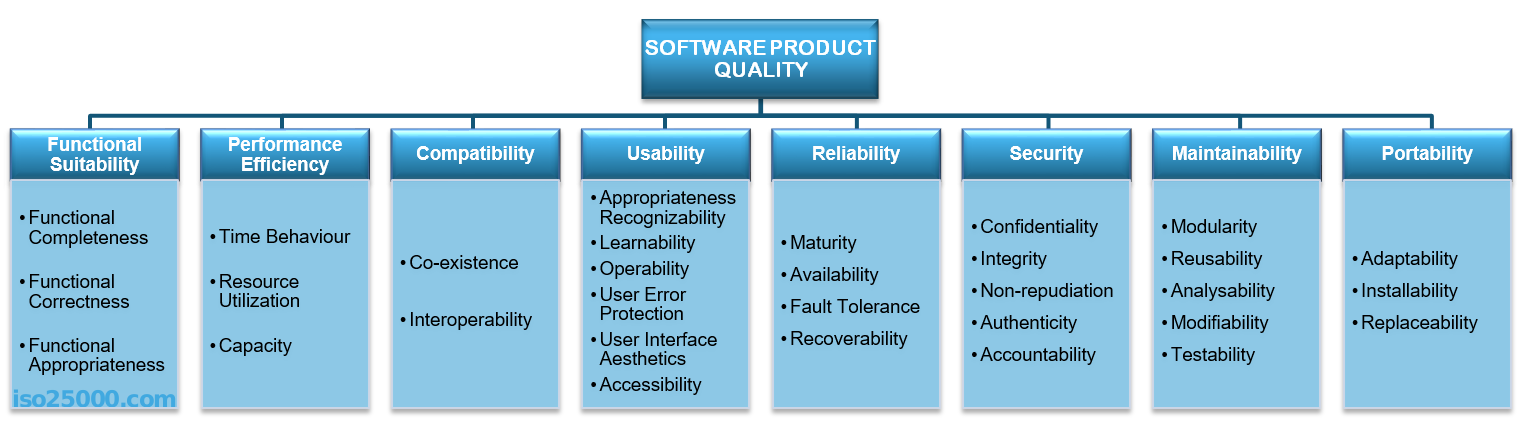
\includegraphics[width=\linewidth]{./images/iso25010.png}
	\caption{Qualitätsattribute einer Software}
	\label{fig:softwareQuality}
	\textit{Quelle: in Anlehnung an \cite{.2022}}
\end{figure}

\noindent
\autoref{fig:softwareQuality} zeigt die acht Charakteristika der Software-Qualität nach ISO / IEC 25010:2011: Funktionalität, Performance, Kompatibilität, Benutzbarkeit, Zuverlässigkeit, Sicherheit, Wartbarkeit und Portierbarkeit. Der Standard bietet ein Framework für die Bewertung der Qualität einer Software an. Er hilft so Software-Produkte zu verbessern und alle Teilbereiche zu beachten, indem der Standard als Leitfaden vom Identifizieren der Anforderungen bis zur Qualitätskontrolle der Software unterstützt.\cite{ISOIEC.}\\

\noindent
Dass IEEE Standard Glossary of Software Engineering Terminology definiert Performance wie folgt:
\begin{quote}
	\emph{\grqq{}The degree to which a system or component accomplishes its designated functions within given constraints, such as speed, accuracy, or memory usage\grqq{}} \cite{IEEE.}
\end{quote}

\noindent
Demnach beschreibt Performance die Reaktion eines Systems auf die Durchführung einer Aktion über einen definierten Zeitraum. Um die Performance einer Software bestimmen zu können, stellt ISO / IEC 25010:2011 drei Charakteristiken zur Verfügung (siehe \autoref{fig:softwareQuality}), die in den folgenden Absätzen beschrieben werden.\\

\noindent
\textbf{Zeitverhalten}\newline
Das Zeitverhalten beschreibt das Maß, in dem die Reaktions-, Verarbeitungszeiten, sowie Durchsatzraten eines Software-Produkts bei der Ausführung definierten Anforderungen entsprechen \cite{ISOIEC.}. Der Fokus liegt hier auf einer schnellen Reaktion der Software, um die definierten Vorgaben für die Performance einzuhalten. Das Zeitverhalten kann durch die Latenz und den Durchsatz genauer spezifiziert werden. Die Latenz definiert ein zeitliches Intervall, in dem die Software eine Antwort auf die Anfrage liefern muss. Dieses Intervall wird in einem Zeitfenster durch eine minimale und maximale Zeitangabe definiert. Die Zeitangaben können absolut oder relativ in Bezug auf ein Event angegeben werden. Die Anzahl an abgeschlossenen Antworten auf eine Anfrage innerhalb eines Beobachtungsintervalls beschreibt den Durchsatz. Daraus kann die Verarbeitungsleistung (Processing Rate) der Software abgeleitet werden. Für eine zuverlässige Angabe ist es empfohlen, mehrere Zeitfenster zu beobachten. Denn es kann sein, dass eine Software 120 Anfragen innerhalb von einer Stunde bearbeiten kann. Dennoch könnte das System versagen, wenn 40 dieser Anfragen innerhalb von drei Minuten abgearbeitet werden müssen.\cite{Barbacci.1995}\\

\noindent
\textbf{Ressourcennutzung}\newline
Das Maß, in dem die Menge und Art der Ressource, die ein Produkt bei der Ausführung seiner Funktionalitäten beansprucht, entspricht der Ressourcennutzung \cite{ISOIEC.}. Es geht um die effiziente Verwaltung der verfügbaren Ressourcen. Dazu zählen die CPU, der Arbeitsspeicher, die Bandbreite des Netzwerks, der Speicherplatz auf der Festplatte und vieles mehr. Die wichtigsten Metriken sind die CPU-Auslastung und der Speicherbedarf sowohl im RAM als auch auf der Festplatte.\cite{Barbacci.1995}\\

\noindent
\textbf{Kapazität}\newline
Die Kapazität beschreibt, inwiefern die maximalen Grenzwerte eines Produkt- oder Systemparameters den Anforderungen entsprechen \cite{ISOIEC.}. Dadurch wird bestimmt, ob das System unter Spitzenlast funktionsfähig bleibt und dadurch skalierbar ist. Hierbei müssen die Anforderungen an die maximale Latenz eingehalten werden. Daher kann die Kapazität alternativ auch als der maximal mögliche Durchsatz unter Einhaltung der gegebenen Latenzanforderungen bezeichnet werden. Das umfasst mehrere Benutzer, die gleichzeitig auf die Software zugreifen, oder größere Transaktionen mit mehr Datenvolumen. Zu den Metriken zählen die maximale Anzahl an gleichzeitigen Benutzern und die maximale Anzahl an möglichen Transaktionen.\cite{Barbacci.1995}

% Performance
% !TeX root = ..\main.tex
\npchapter{Titel 3}

\section{Section 3.1}
TODO

% Kompatibilität
% !TeX root = ..\main.tex
\npchapter{Kompatibilität von Projekten}  \label{compabitility}

\section{Kompatibilität von neuen Projekten} \label{sec:compabitility-newProjects}
TODO \\

\section{Kompatibilität von bestehenden Projekten} \label{sec:compabitility-existingProjects}
TODO \\

\section{Fazit} \label{sec:compabitility-conclusion}
TODO \\

% Schlussbetrachtung
% !TeX root = ..\main.tex
\npchapter{Titel 5}

\section{Section 5.1}
TODO


%Bibliography 
% !TeX root = ..\main.tex
\newpage

% Füge Literaturverzeichnis zum Inhaltsverzeichnis hinzu
\addcontentsline{toc}{chapter}{Bibliography}

% Literaturverzeichnis anstatt Literatur
\renewcommand{\refname}{Bibliography}

\begingroup
%\raggedright
\printbibliography
\endgroup

%Appendix
% !TeX root = ..\main.tex
\appendix
\begin{landscape}
	\chapter{Ergebnisse des Benchmarks} \label{apx:benchmark-results}
	
	\section{HTTP-Server} \label{sec:benchmark-results-http-server}
	\begin{longtable}{
			c
			S[table-format=6.2]
			S[table-format=2.2]
			S[table-format=3.0]
			S[table-format=3]
			S[table-format=2.0]
			S[table-format=4.0]
		}
		\caption{Messungen unter macOS (Bun)}
		\label{tab:macos} \\
		\toprule
		Nr. & {Req/s} & {Durchschn. Latenz (ms)} & {Max. Latenz (ms)} & {Erfolgr. Req (\%)} & {Max. CPU-Ausl. (\%)} & {Max. RAM (kB)} \\
		\midrule
		\endfirsthead
		\toprule
		Nr. & {Bun Req/s} & {Durchschn. Latenz (ms)} & {Max. Latenz (ms)} & {Erfolgr. Req (\%)} & {Max. CPU-Ausl. (\%)} & {Max. RAM (kB)} \\
		\midrule
		\endhead
		1 & 75482.69 & 6.62 & 191 & 100 & 83 & 28928 \\
		2 & 75978.26 & 6.58 & 162 & 100 & 83 & 28960 \\
		3 & 76467.36 & 6.54 & 168 & 100 & 81 & 28832 \\
		4 & 72942.36 & 6.85 & 123 & 100 & 83 & 28992 \\
		5 & 77558.43 & 6.45 & 194 & 100 & 83 & 28800 \\
		Durchschnitt & 75685.82 & 6.61 & 167.7 & 100 & 82.6 & 28902.4 \\
		\bottomrule
	\end{longtable}
	
	\begin{longtable}{
			c
			S[table-format=6.2]
			S[table-format=2.2]
			S[table-format=3.0]
			S[table-format=3]
			S[table-format=2.0]
			S[table-format=4.0]
		}
		\caption{Messungen unter macOS (Node.js LTS)}
		\label{tab:macos-nodejs-lts} \\
		\toprule
		Nr. & {Req/s} & {Durchschn. Latenz (ms)} & {Max. Latenz (ms)} & {Erfolgr. Req (\%)} & {Max. CPU-Ausl. (\%)} & {Max. RAM (kB)} \\
		\midrule
		\endfirsthead
		\toprule
		Nr. & {Req/s} & {Durchschn. Latenz (ms)} & {Max. Latenz (ms)} & {Erfolgr. Req (\%)} & {Max. CPU-Ausl. (\%)} & {Max. RAM (kB)} \\
		\midrule
		\endhead
		1 & 46037.35 & 10.36 & 180 & 100 & 84 & 93536 \\
		2 & 46323.8 & 10.86 & 202 & 100 & 84 & 94432 \\
		3 & 45762.3 & 10.92 & 199 & 100 & 85 & 93456 \\
		4 & 45035.39 & 11.1 & 195 & 100 & 86 & 93584 \\
		5 & 45776.81 & 10.92 & 144 & 100 & 85 & 94016 \\
		Durchschnitt & 45787.13 & 10.83 & 184.6 & 100 & 84.8 & 93804.8 \\
		\bottomrule
	\end{longtable}
	
	\begin{longtable}{
			c
			S[table-format=6.2]
			S[table-format=2.2]
			S[table-format=3.0]
			S[table-format=3]
			S[table-format=2.0]
			S[table-format=4.0]
		}
		\caption{Messungen unter macOS (Node.js Latest)}
		\label{tab:macos-nodejs-current} \\
		\toprule
		Nr. & {Req/s} & {Durchschn. Latenz (ms)} & {Max. Latenz (ms)} & {Erfolgr. Req (\%)} & {Max. CPU-Ausl. (\%)} & {Max. RAM (kB)} \\
		\midrule
		\endfirsthead
		\toprule
		Nr. & {Req/s} & {Durchschn. Latenz (ms)} & {Max. Latenz (ms)} & {Erfolgr. Req (\%)} & {Max. CPU-Ausl. (\%)} & {Max. RAM (kB)} \\
		\midrule
		\endhead
		1 & 45680.37 & 10.94 & 1840 & 100 & 86 & 85584 \\
		2 & 45880.89 & 10.89 & 1860 & 100 & 86 & 85520 \\
		3 & 45939.12 & 10.88 & 1570 & 100 & 85 & 84386 \\
		4 & 45932.14 & 10.88 & 1650 & 100 & 86 & 83616 \\
		5 & 45974.99 & 10.87 & 1120 & 100 & 85 & 85680 \\
		Durchschnitt & 45881.502 & 10.892 & 1608 & 100 & 85.6 & 84957.2 \\
		\bottomrule
	\end{longtable}
	
	\begin{longtable}{
			c
			S[table-format=6.2]
			S[table-format=2.2]
			S[table-format=3.0]
			S[table-format=3]
			S[table-format=2.0]
			S[table-format=5.1]
		}
		\caption{Messungen unter Ubuntu 23.10 (Bun)}
		\label{tab:ubuntu} \\
		\toprule
		Nr. & {Request/s} & {Durchschn. Latenz (ms)} & {Max. Latenz (ms)} & {Erfolgr. Req (\%)} & {Max. CPU-Ausl. (\%)} & {Max. RAM (kB)} \\
		\midrule
		\endfirsthead
		\toprule
		Nr. & {Request/s} & {Durchschn. Latenz (ms)} & {Max. Latenz (ms)} & {Erfolgr. Req (\%)} & {Max. CPU-Ausl. (\%)} & {Max. RAM (kB)} \\
		\midrule
		\endhead
		1 & 103290.25 & 4.84 & 92.06 & 100 & 89 & 47188 \\
		2 & 102852.75 & 4.86 & 120.86 & 100 & 97 & 47608 \\
		3 & 102414.8 & 4.88 & 98.6 & 100 & 96 & 49392 \\
		4 & 103809.8 & 4.81 & 104.46 & 100 & 98 & 47260 \\
		5 & 103707.81 & 4.82 & 99.36 & 100 & 97 & 48484 \\
		Durchschnitt & 103215.082 & 4.842 & 103.068 & 100 & 95.4 & 47986.4 \\
		\bottomrule
	\end{longtable}
	
	\begin{longtable}{
			c
			S[table-format=6.2]
			S[table-format=2.2]
			S[table-format=3.0]
			S[table-format=3]
			S[table-format=2.0]
			S[table-format=5.1]
		}
		\caption{Messungen unter Ubuntu 23.10 (Node.js LTS)}
		\label{tab:ubuntu-nodejs-lts} \\
		\toprule
		Nr. & {Request/s} & {Durchschn. Latenz (ms)} & {Max. Latenz (ms)} & {Erfolgr. Req (\%)} & {Max. CPU-Ausl. (\%)} & {Max. RAM (kB)} \\
		\midrule
		\endfirsthead
		\toprule
		Nr. & {Request/s} & {Durchschn. Latenz (ms)} & {Max. Latenz (ms)} & {Erfolgr. Req (\%)} & {Max. CPU-Ausl. (\%)} & {Max. RAM (kB)} \\
		\midrule
		\endhead
		1 & 30421.51 & 16.44 & 230.8 & 100 & 96 & 93856 \\
		2 & 30448.93 & 16.42 & 208.43 & 100 & 96 & 93212 \\
		3 & 29999.89 & 16.67 & 215.64 & 100 & 95 & 93144 \\
		4 & 30122.16 & 16.59 & 176.54 & 100 & 94 & 92928 \\
		5 & 30488.92 & 16.39 & 199.07 & 100 & 96 & 93116 \\
		Durchschnitt & 30296.282 & 16.502 & 206.096 & 100 & 95.4 & 93251.2 \\
		\bottomrule
	\end{longtable}
	
	\begin{longtable}{
			c
			S[table-format=6.2]
			S[table-format=2.2]
			S[table-format=3.0]
			S[table-format=3]
			S[table-format=2.0]
			S[table-format=5.1]
		}
		\caption{Messungen unter Ubuntu 23.10 (Node.js Current)}
		\label{tab:ubuntu-nodejs-current} \\
		\toprule
		Nr. & {Request/s} & {Durchschn. Latenz (ms)} & {Max. Latenz (ms)} & {Erfolgr. Req (\%)} & {Max. CPU-Ausl. (\%)} & {Max. RAM (kB)} \\
		\midrule
		\endfirsthead
		\toprule
		Nr. & {Request/s} & {Durchschn. Latenz (ms)} & {Max. Latenz (ms)} & {Erfolgr. Req (\%)} & {Max. CPU-Ausl. (\%)} & {Max. RAM (kB)} \\
		\midrule
		\endhead
		1 & 32358.13 & 15.45 & 7960 & 100 & 100 & 86652 \\
		2 & 31700.99 & 15.78 & 8340 & 100 & 90 & 86396 \\
		3 & 32244.05 & 15.51 & 9280 & 100 & 95 & 86280 \\
		4 & 32856.68 & 15.21 & 8210 & 100 & 99 & 86284 \\
		5 & 32269.21 & 15.5 & 8440 & 100 & 98 & 86636 \\
		Durchschnitt & 32285.812 & 15.49 & 8446 & 100 & 96.4 & 86449.6 \\
		\bottomrule
	\end{longtable}
	
\end{landscape}

\begin{landscape}
	\section{Datei-Server} \label{sec:benchmark-results-file-server}
	
	\begin{longtable}{
			c
			S[table-format=6.2]
			S[table-format=2.2]
			S[table-format=3.2]
			S[table-format=3]
			S[table-format=2.0]
			S[table-format=5.0]
		}
		\caption{Messungen unter Ubuntu 23.10 (Bun)}
		\label{tab:ubuntu-various-users} \\
		\toprule
		\multicolumn{7}{c}{50 Benutzer} \\
		Nr. & {Request/s} & {Durchschn. Latenz (ms)} & {Max. Latenz (ms)} & {Erfolgr. Req (\%)} & {Max. CPU-Ausl. (\%)} & {Max. RAM (kB)} \\
		\midrule
		\endfirsthead
		\toprule
		\multicolumn{7}{c}{50 Benutzer} \\
		Nr. & {Request/s} & {Durchschn. Latenz (ms)} & {Max. Latenz (ms)} & {Erfolgr. Req (\%)} & {Max. CPU-Ausl. (\%)} & {Max. RAM (kB)} \\
		\midrule
		\endhead
		1 & 24555.25 & 2.03 & 25.73 & 100 & 98 & 83484 \\
		2 & 24688.31 & 2.02 & 40.45 & 100 & 100 & 82824 \\
		3 & 25083.61 & 1.99 & 30.04 & 100 & 98 & 83876 \\
		4 & 24978.84 & 2 & 25.65 & 100 & 101 & 83756 \\
		5 & 24503.56 & 2.04 & 29.26 & 100 & 98 & 82056 \\
		Durchschnitt & 24761.91 & 2.02 & 30.23 & 100.00 & 99.00 & 83199.20 \\
		\midrule
		\multicolumn{7}{c}{250 Benutzer} \\
		Nr. & {Request/s} & {Durchschn. Latenz (ms)} & {Max. Latenz (ms)} & {Erfolgr. Req (\%)} & {Max. CPU-Ausl. (\%)} & {Max. RAM (kB)} \\
		\midrule
		1 & 24585.85 & 10.17 & 100.97 & 100 & 98 & 82372 \\
		2 & 24988.13 & 10 & 96.19 & 100 & 97 & 83272 \\
		3 & 24290.11 & 10.29 & 73.98 & 100 & 97 & 83132 \\
		4 & 24399.87 & 10.24 & 105.26 & 100 & 98 & 82808 \\
		5 & 24926.9 & 10.03 & 80.57 & 100 & 97 & 84088 \\
		Durchschnitt & 24638.17 & 10.15 & 91.39 & 100.00 & 97.40 & 83134.40 \\
		\midrule
		\multicolumn{7}{c}{500 Benutzer} \\
		Nr. & {Request/s} & {Durchschn. Latenz (ms)} & {Max. Latenz (ms)} & {Erfolgr. Req (\%)} & {Max. CPU-Ausl. (\%)} & {Max. RAM (kB)} \\
		\midrule
		1 & 23899.18 & 20.91 & 116.19 & 100 & 96 & 82128 \\
		2 & 24201.74 & 20.65 & 108.4 & 100 & 96 & 83196 \\
		3 & 24153.93 & 20.69 & 115.38 & 100 & 100 & 82692 \\
		4 & 23658.7 & 21.12 & 119.64 & 100 & 98 & 82672 \\
		5 & 24399.08 & 20.5 & 117.62 & 100 & 99 & 82948 \\
		Durchschnitt & 24155.31 & 20.69 & 116.36 & 100.00 & 98.40 & 83124.80 \\
		\midrule
		\multicolumn{7}{c}{1000 Benutzer} \\
		Nr. & {Request/s} & {Durchschn. Latenz (ms)} & {Max. Latenz (ms)} & {Erfolgr. Req (\%)} & {Max. CPU-Ausl. (\%)} & {Max. RAM (kB)} \\
		\midrule
		1 & 23963.96 & 41.81 & 1230 & 100 & 98 & 82180 \\
		2 & 23684.71 & 42.25 & 1160 & 100 & 95 & 81876 \\
		3 & 23702.16 & 42.25 & 1170 & 100 & 93 & 83052 \\
		4 & 23546.82 & 42.53 & 1160 & 100 & 98 & 82880 \\
		5 & 24036.35 & 41.63 & 1130 & 100 & 97 & 83320 \\
		Durchschnitt & 23786.80 & 42.09 & 1170.00 & 100.00 & 96.20 & 82661.60 \\
		\bottomrule
	\end{longtable}
	
	\begin{longtable}{
			c
			S[table-format=6.2]
			S[table-format=2.2]
			S[table-format=3.2]
			S[table-format=3]
			S[table-format=2.0]
			S[table-format=5.0]
		}
		\caption{Messungen unter Node.js LTS auf Ubuntu 23.10}
		\label{tab:nodejs-measurements}
		\\
		\toprule
		\multicolumn{7}{c}{50 Benutzer} \\
		Nr. & {Request/s} & {Durchschn. Latenz (ms)} & {Max. Latenz (ms)} & {Erfolgr. Req (\%)} & {Max. CPU-Ausl. (\%)} & {Max. RAM (kB)} \\
		\midrule
		\endfirsthead
		\toprule
		\multicolumn{7}{c}{50 Benutzer} \\
		Nr. & {Request/s} & {Durchschn. Latenz (ms)} & {Max. Latenz (ms)} & {Erfolgr. Req (\%)} & {Max. CPU-Ausl. (\%)} & {Max. RAM (kB)} \\
		\midrule
		\endhead
		1 & 11853.46 & 4.22 & 78.54 & 100 & 137 & 69480 \\
		2 & 11924.96 & 4.08 & 71.56 & 100 & 135 & 71184 \\
		3 & 12253.47 & 4.08 & 71.51 & 100 & 135 & 74640 \\
		4 & 11806.59 & 4.23 & 64.23 & 100 & 134 & 71224 \\
		5 & 11819.12 & 4.23 & 73.19 & 100 & 133 & 76260 \\
		Durchschnitt & 11931.52 & 4.17 & 71.81 & 100.00 & 134.80 & 72557.60 \\
		\midrule
		\multicolumn{7}{c}{250 Benutzer} \\
		Nr. & {Request/s} & {Durchschn. Latenz (ms)} & {Max. Latenz (ms)} & {Erfolgr. Req (\%)} & {Max. CPU-Ausl. (\%)} & {Max. RAM (kB)} \\
		\midrule
		1 & 9454.04 & 26.38 & 249.57 & 100 & 169 & 115504 \\
		2 & 9395.36 & 26.55 & 221.37 & 100 & 169 & 121036 \\
		3 & 9276.2 & 26.89 & 215.68 & 100 & 173 & 112908 \\
		4 & 9379.2 & 26.59 & 192.39 & 100 & 167 & 122620 \\
		5 & 9362.02 & 26.64 & 223.04 & 100 & 171 & 114472 \\
		Durchschnitt & 9373.36 & 26.61 & 220.41 & 100.00 & 169.80 & 117308.00 \\
		\midrule
		\multicolumn{7}{c}{500 Benutzer} \\
		Nr. & {Request/s} & {Durchschn. Latenz (ms)} & {Max. Latenz (ms)} & {Erfolgr. Req (\%)} & {Max. CPU-Ausl. (\%)} & {Max. RAM (kB)} \\
		\midrule
		1 & 7650.31 & 64.53 & 287.7 & 100 & 166 & 105356 \\
		2 & 8460.46 & 58.41 & 305.46 & 100 & 176 & 106928 \\
		3 & 8428.35 & 58.51 & 285.69 & 100 & 166 & 103704 \\
		4 & 8292.37 & 59.61 & 313.21 & 100 & 171 & 106108 \\
		5 & 8410.83 & 58.73 & 292.88 & 100 & 165 & 104264 \\
		Durchschnitt & 8398.00 & 58.82 & 299.31 & 100.00 & 169.50 & 105251.00 \\
		\midrule
		\multicolumn{7}{c}{1000 Benutzer} \\
		Nr. & {Request/s} & {Durchschn. Latenz (ms)} & {Max. Latenz (ms)} & {Erfolgr. Req (\%)} & {Max. CPU-Ausl. (\%)} & {Max. RAM (kB)} \\
		\midrule
		1 & 8491.34 & 118.31 & 1260 & 100 & 170 & 140472 \\
		2 & 7656.16 & 130.42 & 1260 & 100 & 178 & 143180 \\
		3 & 7714.78 & 129.42 & 1270 & 100 & 160 & 178588 \\
		4 & 8174.67 & 123.02 & 1270 & 100 & 152 & 149484 \\
		5 & 7698.82 & 129.62 & 1260 & 100 & 177 & 147612 \\
		Durchschnitt & 7947.15 & 126.16 & 1264.00 & 100.00 & 167.40 & 151867.20 \\
		\bottomrule
	\end{longtable}
	
	\begin{longtable}{
			c
			S[table-format=6.2]
			S[table-format=2.2]
			S[table-format=3.2]
			S[table-format=3]
			S[table-format=2.0]
			S[table-format=6.0]
		}
		\caption{Messungen unter Node.js Latest auf Ubuntu 23.10}
		\label{tab:nodejs-latest-measurements}
		\\
		\toprule
		\multicolumn{7}{c}{50 Benutzer} \\
		Nr. & {Request/s} & {Durchschn. Latenz (ms)} & {Max. Latenz (ms)} & {Erfolgr. Req (\%)} & {Max. CPU-Ausl. (\%)} & {Max. RAM (kB)} \\
		\midrule
		\endfirsthead
		\toprule
		\multicolumn{7}{c}{50 Benutzer} \\
		Nr. & {Request/s} & {Durchschn. Latenz (ms)} & {Max. Latenz (ms)} & {Erfolgr. Req (\%)} & {Max. CPU-Ausl. (\%)} & {Max. RAM (kB)} \\
		\midrule
		\endhead
		1 & 14237.06 & 3.51 & 116.84 & 100 & 174 & 88056 \\
		2 & 14305.85 & 3.49 & 135.14 & 100 & 194 & 84784 \\
		3 & 14685.7 & 3.4 & 146.92 & 100 & 193 & 82028 \\
		4 & 14253.49 & 3.51 & 161.68 & 100 & 193 & 85144 \\
		5 & 14690.78 & 3.4 & 127.55 & 100 & 197 & 86808 \\
		Durchschnitt & 14434.58 & 3.46 & 137.63 & 100.00 & 190.20 & 85364.00 \\
		\midrule
		\multicolumn{7}{c}{250 Benutzer} \\
		Nr. & {Request/s} & {Durchschn. Latenz (ms)} & {Max. Latenz (ms)} & {Erfolgr. Req (\%)} & {Max. CPU-Ausl. (\%)} & {Max. RAM (kB)} \\
		\midrule
		1 & 12075.16 & 20.7 & 860 & 100 & 222 & 128460 \\
		2 & 12006.8 & 20.81 & 816.63 & 100 & 218 & 124552 \\
		3 & 12038.16 & 20.76 & 880 & 100 & 220 & 121192 \\
		4 & 11927.89 & 20.95 & 845.54 & 100 & 221 & 121700 \\
		5 & 12158.18 & 20.56 & 860 & 100 & 221 & 121488 \\
		Durchschnitt & 12041.24 & 20.76 & 852.43 & 100.00 & 220.40 & 123478.40 \\
		\midrule
		\multicolumn{7}{c}{500 Benutzer} \\
		Nr. & {Request/s} & {Durchschn. Latenz (ms)} & {Max. Latenz (ms)} & {Erfolgr. Req (\%)} & {Max. CPU-Ausl. (\%)} & {Max. RAM (kB)} \\
		\midrule
		1 & 10322.75 & 47.96 & 1710 & 100 & 268 & 172996 \\
		2 & 10462.03 & 47.33 & 1740 & 100 & 265 & 118604 \\
		3 & 10337.76 & 47.97 & 1770 & 100 & 250 & 174576 \\
		4 & 10478.85 & 47.32 & 1740 & 100 & 264 & 175628 \\
		5 & 10254 & 48.39 & 1740 & 100 & 262 & 175036 \\
		Durchschnitt & 10383.16 & 47.75 & 1747.50 & 100.00 & 260.25 & 160961.00 \\
		\midrule
		\multicolumn{7}{c}{1000 Benutzer} \\
		Nr. & {Request/s} & {Durchschn. Latenz (ms)} & {Max. Latenz (ms)} & {Erfolgr. Req (\%)} & {Max. CPU-Ausl. (\%)} & {Max. RAM (kB)} \\
		\midrule
		1 & 8535.43 & 116.42 & 4240 & 100 & 278 & 213864 \\
		2 & 8553.51 & 116.28 & 3810 & 100 & 279 & 209776 \\
		3 & 8573.22 & 115.88 & 4240 & 100 & 277 & 209276 \\
		4 & 8655.02 & 114.96 & 4100 & 100 & 281 & 211692 \\
		5 & 8630.1 & 115.3 & 4070 & 100 & 283 & 213220 \\
		Durchschnitt & 8589.46 & 115.77 & 4092.00 & 100.00 & 279.60 & 211565.60 \\
		\bottomrule
	\end{longtable}
	
	\begin{longtable}{
			c
			S[table-format=6.2]
			S[table-format=2.2]
			S[table-format=3.2]
			S[table-format=3]
			S[table-format=2.0]
			S[table-format=6.0]
		}
		\caption{Messungen unter Node.js Latest auf macOS}
		\label{tab:nodejs-macos-measurements}
		\\
		\toprule
		\multicolumn{7}{c}{50 Benutzer} \\
		Nr. & {Request/s} & {Durchschn. Latenz (ms)} & {Max. Latenz (ms)} & {Erfolgr. Req (\%)} & {Max. CPU-Ausl. (\%)} & {Max. RAM (kB)} \\
		\midrule
		\endfirsthead
		\toprule
		\multicolumn{7}{c}{50 Benutzer} \\
		Nr. & {Request/s} & {Durchschn. Latenz (ms)} & {Max. Latenz (ms)} & {Erfolgr. Req (\%)} & {Max. CPU-Ausl. (\%)} & {Max. RAM (kB)} \\
		\midrule
		\endhead
		1 & 25276.77 & 1.98 & 18.82 & 100 & 92 & 67328 \\
		2 & 25302.77 & 1.97 & 14.4 & 100 & 94 & 65744 \\
		3 & 25293.36 & 1.98 & 14.06 & 100 & 95 & 65840 \\
		4 & 25292.46 & 1.98 & 13.51 & 100 & 93 & 65956 \\
		5 & 25330.78 & 1.97 & 16.1 & 100 & 94 & 654230 \\
		Durchschnitt & 25299.23 & 1.98 & 15.38 & 100.00 & 93.60 & 183819.60 \\
		\midrule
		\multicolumn{7}{c}{250 Benutzer} \\
		Nr. & {Request/s} & {Durchschn. Latenz (ms)} & {Max. Latenz (ms)} & {Erfolgr. Req (\%)} & {Max. CPU-Ausl. (\%)} & {Max. RAM (kB)} \\
		\midrule
		1 & 25464.61 & 9.82 & 55.58 & 100 & 89 & 66698 \\
		2 & 25435.68 & 9.83 & 52.12 & 100 & 92 & 66384 \\
		3 & 25476.74 & 9.81 & 50.91 & 100 & 93 & 66464 \\
		4 & 25372.19 & 9.85 & 49.03 & 100 & 92 & 66640 \\
		5 & 25451.01 & 9.82 & 49.88 & 100 & 93 & 66560 \\
		Durchschnitt & 25440.05 & 9.83 & 51.50 & 100.00 & 91.80 & 66549.20 \\
		\midrule
		\multicolumn{7}{c}{500 Benutzer} \\
		Nr. & {Request/s} & {Durchschn. Latenz (ms)} & {Max. Latenz (ms)} & {Erfolgr. Req (\%)} & {Max. CPU-Ausl. (\%)} & {Max. RAM (kB)} \\
		\midrule
		1 & 23707.59 & 21.08 & 195.63 & 100 & 90 & 64264 \\
		2 & 23920.81 & 20.9 & 239.5 & 100 & 86 & 65040 \\
		3 & 23909.89 & 20.9 & 204.46 & 100 & 90 & 65024 \\
		4 & 23825.78 & 20.98 & 206.59 & 100 & 89 & 64880 \\
		5 & 23879.56 & 20.93 & 220.08 & 100 & 90 & 64880 \\
		Durchschnitt & 23848.73 & 20.96 & 213.25 & 100.00 & 89.00 & 64817.60 \\
		\midrule
		\multicolumn{7}{c}{1000 Benutzer} \\
		Nr. & {Request/s} & {Durchschn. Latenz (ms)} & {Max. Latenz (ms)} & {Erfolgr. Req (\%)} & {Max. CPU-Ausl. (\%)} & {Max. RAM (kB)} \\
		\midrule
		1 & 24846.18 & 40.22 & 451.41 & 99.96 & 91 & 68192 \\
		2 & 24776.04 & 40.34 & 466.86 & 99.95 & 90 & 67472 \\
		3 & 24789.88 & 40.38 & 479.3 & 99.95 & 91 & 67280 \\
		4 & 24746.3 & 40.38 & 479.3 & 99.96 & 90 & 6824 \\
		5 & 24773.9 & 40.34 & 462.65 & 99.96 & 91 & 67952 \\
		Durchschnitt & 24786.46 & 40.33 & 467.90 & 99.96 & 90.60 & 55544.00 \\
		\bottomrule
	\end{longtable}
	
	\begin{longtable}{
			c
			S[table-format=5.2]
			S[table-format=2.2]
			S[table-format=2.2]
			S[table-format=3]
			S[table-format=3.0]
			S[table-format=6.0]
		}
		\caption{Messungen unter Node.js LTS auf macOS}
		\label{tab:nodejs-lts-macos-measurements}
		\\
		\toprule
		\multicolumn{7}{c}{50 Benutzer} \\
		Nr. & {Request/s} & {Durchschn. Latenz (ms)} & {Max. Latenz (ms)} & {Erfolgr. Req (\%)} & {Max. CPU-Ausl. (\%)} & {Max. RAM (kB)} \\
		\midrule
		\endfirsthead
		\toprule
		\multicolumn{7}{c}{50 Benutzer} \\
		Nr. & {Request/s} & {Durchschn. Latenz (ms)} & {Max. Latenz (ms)} & {Erfolgr. Req (\%)} & {Max. CPU-Ausl. (\%)} & {Max. RAM (kB)} \\
		\midrule
		\endhead
		1 & 21515 & 2.32 & 33.96 & 100 & 146 & 120544 \\
		2 & 19785.3 & 2.53 & 36.05 & 100 & 142 & 125616 \\
		3 & 19363.94 & 2.58 & 33.9 & 100 & 143 & 124096 \\
		4 & 21722.08 & 2.3 & 29.84 & 100 & 143 & 109568 \\
		5 & 21449.79 & 2.33 & 33.51 & 100 & 145 & 119792 \\
		Durchschnitt & 20767.22 & 2.41 & 33.45 & 100.00 & 143.80 & 119923.20 \\
		\midrule
		\multicolumn{7}{c}{250 Benutzer} \\
		Nr. & {Request/s} & {Durchschn. Latenz (ms)} & {Max. Latenz (ms)} & {Erfolgr. Req (\%)} & {Max. CPU-Ausl. (\%)} & {Max. RAM (kB)} \\
		\midrule
		1 & 15917.54 & 15.55 & 70.35 & 100 & 193 & 195552 \\
		2 & 16075.37 & 15.51 & 81.9 & 100 & 186 & 168992 \\
		3 & 16074.26 & 15.55 & 65.21 & 100 & 189 & 191920 \\
		4 & 16111.43 & 15.51 & 81.9 & 100 & 188 & 189536 \\
		5 & 15924.32 & 15.7 & 70.46 & 100 & 191 & 176272 \\
		Durchschnitt & 16020.58 & 15.56 & 73.96 & 100.00 & 189.40 & 184454.40 \\
		\midrule
		\multicolumn{7}{c}{500 Benutzer} \\
		Nr. & {Request/s} & {Durchschn. Latenz (ms)} & {Max. Latenz (ms)} & {Erfolgr. Req (\%)} & {Max. CPU-Ausl. (\%)} & {Max. RAM (kB)} \\
		\midrule
		1 & 14317.65 & 34.93 & 248.08 & 100 & 189 & 229776 \\
		2 & 14508.2 & 34.46 & 231.62 & 100 & 197 & 198496 \\
		3 & 14466.72 & 34.56 & 214.82 & 100 & 185 & 208496 \\
		4 & 14610.55 & 34.21 & 198.59 & 100 & 176 & 212880 \\
		5 & 14647.9 & 34.12 & 238.61 & 100 & 190 & 209896 \\
		Durchschnitt & 14510.20 & 34.46 & 226.34 & 100.00 & 187.40 & 211908.80 \\
		\midrule
		\multicolumn{7}{c}{1000 Benutzer} \\
		Nr. & {Request/s} & {Durchschn. Latenz (ms)} & {Max. Latenz (ms)} & {Erfolgr. Req (\%)} & {Max. CPU-Ausl. (\%)} & {Max. RAM (kB)} \\
		\midrule
		1 & 14970.63 & 66.75 & 511.17 & 99.92 & 193 & 284000 \\
		2 & 14629.17 & 68.36 & 452.81 & 99.93 & 198 & 300096 \\
		3 & 14524.19 & 68.75 & 594.74 & 99.92 & 195 & 286704 \\
		4 & 14274.59 & 69.98 & 572.31 & 99.92 & 199 & 294704 \\
		5 & 13378.25 & 74.77 & 550.02 & 99.92 & 190 & 311296 \\
		Durchschnitt & 14355.37 & 69.72 & 536.21 & 99.92 & 195.00 & 295360.00 \\
		\bottomrule
	\end{longtable}
	
	\begin{longtable}{
			c
			S[table-format=5.2]
			S[table-format=2.2]
			S[table-format=2.2]
			S[table-format=3]
			S[table-format=3.0]
			S[table-format=6.0]
		}
		\caption{Messungen unter Node.js Latest auf macOS}
		\label{tab:nodejs-latest-macos-measurements}
		\\
		\toprule
		\multicolumn{7}{c}{50 Benutzer} \\
		Nr. & {Request/s} & {Durchschn. Latenz (ms)} & {Max. Latenz (ms)} & {Erfolgr. Req (\%)} & {Max. CPU-Ausl. (\%)} & {Max. RAM (kB)} \\
		\midrule
		\endfirsthead
		\toprule
		\multicolumn{7}{c}{50 Benutzer} \\
		Nr. & {Request/s} & {Durchschn. Latenz (ms)} & {Max. Latenz (ms)} & {Erfolgr. Req (\%)} & {Max. CPU-Ausl. (\%)} & {Max. RAM (kB)} \\
		\midrule
		\endhead
		1 & 21553.66 & 2.32 & 81.25 & 100 & 146 & 117296 \\
		2 & 21499.51 & 2.32 & 61.8 & 100 & 148 & 109888 \\
		3 & 21808.63 & 2.29 & 61.93 & 100 & 146 & 112464 \\
		4 & 21799.37 & 2.29 & 63.66 & 100 & 144 & 119520 \\
		5 & 21519.05 & 2.32 & 60.17 & 100 & 148 & 115120 \\
		Durchschnitt & 21636.04 & 2.31 & 65.76 & 100.00 & 146.40 & 114857.60 \\
		\midrule
		\multicolumn{7}{c}{250 Benutzer} \\
		Nr. & {Request/s} & {Durchschn. Latenz (ms)} & {Max. Latenz (ms)} & {Erfolgr. Req (\%)} & {Max. CPU-Ausl. (\%)} & {Max. RAM (kB)} \\
		\midrule
		1 & 17388.28 & 14.38 & 469.75 & 99.99 & 190 & 203264 \\
		2 & 17301.54 & 14.45 & 484.46 & 99.99 & 191 & 202544 \\
		3 & 17374.5 & 14.39 & 455.17 & 100.00 & 186 & 184224 \\
		4 & 17193.03 & 14.54 & 478.6 & 99.99 & 186 & 208992 \\
		5 & 16918.4 & 5.55 & 492.5 & 100.00 & 187 & 198144 \\
		Durchschnitt & 17235.15 & 12.66 & 476.10 & 99.99 & 188.00 & 199433.60 \\
		\midrule
		\multicolumn{7}{c}{500 Benutzer} \\
		Nr. & {Request/s} & {Durchschn. Latenz (ms)} & {Max. Latenz (ms)} & {Erfolgr. Req (\%)} & {Max. CPU-Ausl. (\%)} & {Max. RAM (kB)} \\
		\midrule
		1 & 14790.27 & 33.81 & 1720 & 99.50 & 195 & 221728 \\
		2 & 14729.2 & 33.93 & 1790 & 99.40 & 194 & 219552 \\
		3 & 14749.95 & 33.91 & 1649 & 99.70 & 198 & 234800 \\
		4 & 14722.22 & 33.98 & 1920 & 99.40 & 193 & 243920 \\
		5 & 14628.28 & 34.14 & 1820 & 99.70 & 194 & 257200 \\
		Durchschnitt & 14723.98 & 33.95 & 1779.80 & 99.54 & 194.80 & 235440.00 \\
		\midrule
		\multicolumn{7}{c}{1000 Benutzer} \\
		Nr. & {Request/s} & {Durchschn. Latenz (ms)} & {Max. Latenz (ms)} & {Erfolgr. Req (\%)} & {Max. CPU-Ausl. (\%)} & {Max. RAM (kB)} \\
		\midrule
		1 & 14937.53 & 66.91 & 6000 & 99.87 & 210 & 283264 \\
		2 & 14518.01 & 68.83 & 5140 & 99.48 & 206 & 366512 \\
		3 & 14594.26 & 67.85 & 4350 & 99.46 & 203 & 317392 \\
		4 & 14719.55 & 68.2 & 4540 & 99.38 & 198 & 361280 \\
		5 & 14651.76 & 68.2 & 4540 & 99.50 & 206 & 323952 \\
		Durchschnitt & 14684.22 & 68.00 & 4914.00 & 99.54 & 204.60 & 330480.00 \\
		\bottomrule
	\end{longtable}
	
	\section{Fibonacci-Folge} \label{sec:benchmark-results-fibonacci}
	\begin{longtable}{c S[table-format=2.2] c S[table-format=5.0]}
		\caption{Messungen unter MacOS} \\
		\toprule
		\multicolumn{4}{c}{Bun} \\
		Nr. & {Ausführungszeit (s)} & {CPU-Auslastung} & {Maximale RAM-Nutzung (kbytes)} \\
		\midrule
		\endfirsthead
		\toprule
		\multicolumn{4}{c}{Bun} \\
		Nr. & {Ausführungszeit (s)} & {CPU-Auslastung} & {Maximale RAM-Nutzung (kbytes)} \\
		\midrule
		\endhead
		1 & 3,23 & 100 & 25840 \\
		2 & 3,23 & 100 & 25776 \\
		3 & 3,24 & 100 & 25904 \\
		4 & 3,26 & 100 & 26160 \\
		5 & 3,26 & 100 & 25952 \\
		Durchschnitt & 3,24 & 100,00 & 25926,40 \\
		\midrule
		\multicolumn{4}{c}{Node.js LTS} \\
		Nr. & {Ausführungszeit (s)} & {CPU-Auslastung} & {Maximale RAM-Nutzung (kbytes)} \\
		\midrule
		1 & 6,56 & 99 & 42496 \\
		2 & 6,5 & 99 & 40976 \\
		3 & 6,48 & 99 & 40848 \\
		4 & 6,5 & 99 & 42448 \\
		5 & 6,49 & 99 & 43120 \\
		Durchschnitt & 6,51 & 99,00 & 41977,60 \\
		\midrule
		\multicolumn{4}{c}{Node.js Latest} \\
		Nr. & {Ausführungszeit (s)} & {CPU-Auslastung} & {Maximale RAM-Nutzung (kbytes)} \\
		\midrule
		1 & 6,32 & 99 & 36688 \\
		2 & 6,32 & 99 & 36608 \\
		3 & 6,32 & 99 & 36912 \\
		4 & 6,32 & 99 & 36800 \\
		5 & 6,33 & 99 & 36672 \\
		Durchschnitt & 6,32 & 99,00 & 36736,00 \\
		\bottomrule
	\end{longtable}	
	
	\begin{longtable}{c S[table-format=2.2] c S[table-format=5.0]}
		\caption{Messungen unter Ubuntu 23.10} \\
		\toprule
		\multicolumn{4}{c}{Bun} \\
		Nr. & {Ausführungszeit (s)} & {CPU-Auslastung} & {Maximale RAM-Nutzung (kbytes)} \\
		\midrule
		\endfirsthead
		\toprule
		\multicolumn{4}{c}{Bun} \\
		Nr. & {Ausführungszeit (s)} & {CPU-Auslastung} & {Maximale RAM-Nutzung (kbytes)} \\
		\midrule
		\endhead
		1 & 4,48 & 100 & 44624 \\
		2 & 4,49 & 100 & 45644 \\
		3 & 4,46 & 100 & 45380 \\
		4 & 4,47 & 100 & 44744 \\
		5 & 4,46 & 100 & 43844 \\
		Durchschnitt & 4,47 & 100,00 & 44847,20 \\
		\midrule
		\multicolumn{4}{c}{Node.js LTS} \\
		Nr. & {Ausführungszeit (s)} & {CPU-Auslastung} & {Maximale RAM-Nutzung (kbytes)} \\
		\midrule
		1 & 7,39 & 98 & 45696 \\
		2 & 7,29 & 99 & 46336 \\
		3 & 7,35 & 100 & 46336 \\
		4 & 7,29 & 99 & 46336 \\
		5 & 7,41 & 100 & 46080 \\
		Durchschnitt & 7,35 & 99,20 & 46156,80 \\
		\midrule
		\multicolumn{4}{c}{Node.js Latest} \\
		Nr. & {Ausführungszeit (s)} & {CPU-Auslastung} & {Maximale RAM-Nutzung (kbytes)} \\
		\midrule
		1 & 7,19 & 100 & 43904 \\
		2 & 7,17 & 100 & 43904 \\
		3 & 7,17 & 100 & 43776 \\
		4 & 7,17 & 99 & 43776 \\
		5 & 7,2 & 99 & 43776 \\
		Durchschnitt & 7,18 & 99,60 & 43827,20 \\
		\bottomrule
	\end{longtable}
\end{landscape}

\section{Zusätzliche Diagramme} \label{sec:benchmark-results-diagrams}
\begin{figure}[h!]
	\centering
	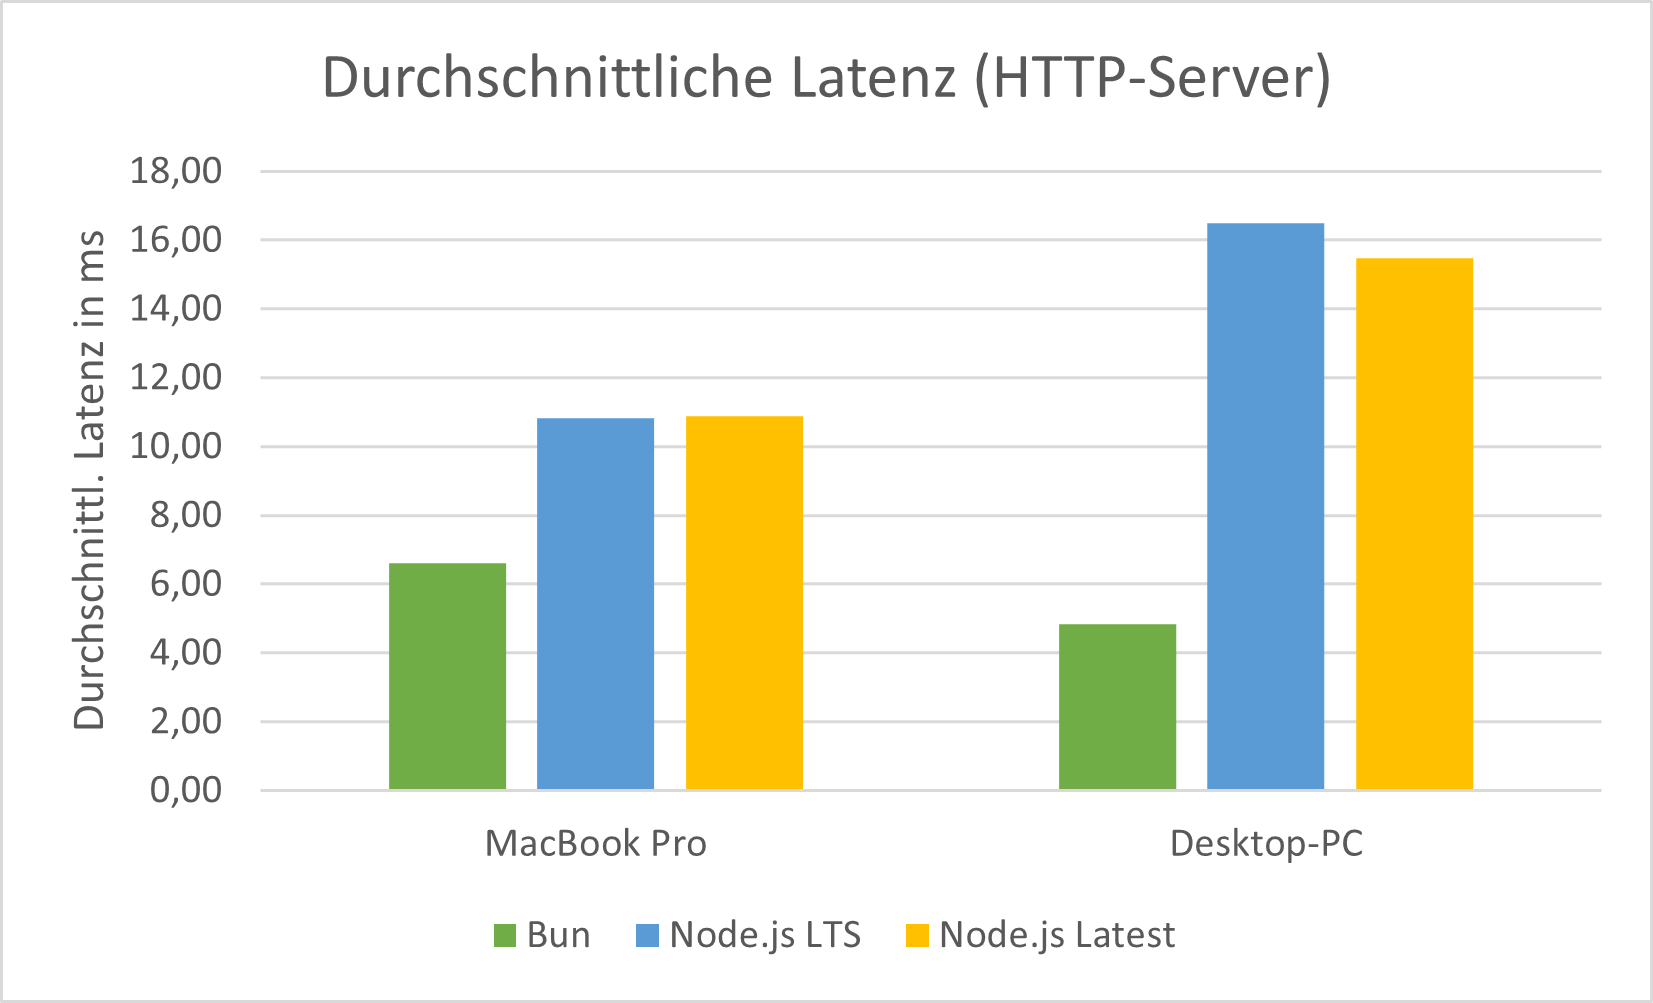
\includegraphics[width=\linewidth]{./images/httpServerAverageLatency.png}
	\caption{Ausführungszeit für die Berechnung der Fibonacci-Folge}
	\label{fig:httpServerAverageLatency}
\end{figure}



\end{document}